\documentclass[11pt]{article}

\usepackage[a4paper,margin=1in]{geometry}
\usepackage[T1]{fontenc}
\usepackage{microtype}
\usepackage{amsmath,amssymb,amsthm}
\usepackage{graphicx}
\usepackage{booktabs}
\usepackage{xcolor}
\usepackage{enumitem}
\usepackage{verbatim}
\usepackage[colorlinks=true,allcolors=blue]{hyperref}
\usepackage{natbib}
\bibliographystyle{plainnat}

\newtheorem{proposition}{Proposition}

\title{\textbf{ThermoGuard: Real-Time Indoor Heat Risk Forecasting\\for Vulnerable Housing under Extreme Heat Events}}
\author{Anwar Debes\\
University of Agder \\
\texttt{anwar@uia.no}\\
\vspace{0.5em}
\small Draft v0.1, May 2026
}
\date{}

\begin{document}
\maketitle

\begin{abstract}
Heatwaves are now the deadliest weather hazard in much of the world: the August 2003 European heatwave killed approximately 70{,}000 people \citep{poumadere2005french}; the July 1995 Chicago heatwave killed 700+ in a single city in five days \citep{semenza1996chicago}; the June 2021 Pacific Northwest heat dome killed an estimated 1{,}400 across Oregon, Washington and British Columbia, with body counts dominated by elderly low-income residents without air conditioning \citep{philip2021pnw}.  Most heat-health warning systems today issue \emph{outdoor} forecasts, but the documented mortality is overwhelmingly indoor, in homes whose temperatures lag the outdoors by 12--24 hours and depend critically on building physics, AC access, and occupant vulnerability.  Recent literature \citep{iato2025,indoorvulnerability2025,taylor2018london} establishes the need for indoor-aware warnings but has so far produced offline building-simulation studies rather than real-time deployable systems.\\

\noindent We introduce \textbf{ThermoGuard}, the first end-to-end real-time pipeline for hyperlocal indoor heat-risk forecasting and equity-aware triage of public-health interventions.  Four contributions:

(i) a 2R--2C lumped-capacitance physics model of indoor temperature, parametrised by five residential archetypes spanning the documented vulnerability stratification (low-income pre-1980 no-AC, midcentury walkup with window-AC, modern central-AC, care home top-floor no-AC, tropical slum dwelling);

(ii) a hybrid physics+ML forecaster that combines the RC backbone with a closed-form ridge residual learner -- runs on a single CPU, deterministic latency, deployable at city scale every 10 minutes;

(iii) a per-resident heat-mortality risk model that integrates Steadman heat index \citep{steadman1979heatindex}, Stull wet-bulb-globe-temperature \citep{stull2011wetbulb}, age-band epidemiology, chronic conditions, mobility, AC access, social isolation, and income quintile, calibrated against documented heatwave excess mortality;

(iv) an equity-aware triage optimiser that allocates limited intervention budgets (cooling-center visits, hydration kits) under a per-stratum equity floor, quantifying the tradeoff between aggregate lives saved and per-stratum coverage.

\noindent We evaluate on three reference heatwaves -- PNW 2021, European 2003, Chicago 1995 -- with a synthetic 1{,}500-household city reflecting documented vulnerability mix.  Headline results: the system reproduces documented mortality concentration (top-25\% of households account for 70--82\% of expected deaths), the hybrid forecaster matches the physics ground truth within $0.5$~$^\circ$C MAE and \emph{beats} the physics-only baseline on the high-humidity Chicago 1995 event ($1.69$ vs $2.07$~$^\circ$C MAE), and the equity-aware allocator achieves $64\%$ of the greedy allocator's raw lives saved while delivering $11\%$ minimum stratum coverage where greedy yields zero.  The full pipeline runs in under three minutes on a single CPU for a 1{,}500-household city.  We discuss honestly where the system does and does not yet earn its keep (Section~\ref{sec:limits}), including the well-known limitation that under perfect physics simulators a pure-physics forecaster matches the ground truth by construction, and outline the path to live deployment with Ecobee-class smart thermostat ingestion.
\end{abstract}

\section{Introduction}

Heatwaves are the deadliest natural hazard in most of the developed world, and the gap is widening as climate change intensifies the events while urbanisation concentrates vulnerable populations \citep{ebi2021climateheath}.  Three reference events bracket the empirical range:

\begin{itemize}[leftmargin=2em]
\item \textbf{Chicago 1995} (5 days, T peak $\approx 40^\circ$C, RH 65\%): 739 documented deaths \citep{semenza1996chicago, kaiser2007chicago}; mortality concentrated in elderly residents of top-floor apartments without AC.
\item \textbf{European 2003} (10+ days, T peak $\approx 39^\circ$C, RH 45\%): $\approx 70{,}000$ deaths across continental Europe \citep{poumadere2005french}; mortality concentrated in care-home residents and low-income elderly.
\item \textbf{Pacific Northwest 2021} (3 days, T peak $\approx 46^\circ$C, RH 30\%): $\approx 1{,}400$ deaths in a region with $<10\%$ AC penetration \citep{philip2021pnw}; mortality concentrated in low-income elderly without home AC.
\end{itemize}

What unites the three events is not the outdoor temperature but the indoor temperature in poorly-ventilated, no-AC housing inhabited by physiologically vulnerable people.  The outdoor temperature is the public-facing forecast variable in essentially every operational heat-health warning system today; the indoor temperature is the variable that actually drives mortality.

\paragraph{Why the gap is hard to close.}  Building physics is well-understood; the WHO Housing and Health Guidelines \citep{whoheat2018} document the relevant equations.  But operational HHWS face four constraints:

\begin{enumerate}[leftmargin=2em]
\item No real-time indoor measurements at city scale (smart-thermostat coverage is $<20\%$ of US households and biased toward higher incomes -- the wrong tail).
\item Need to forecast hours-to-days ahead, not just nowcast.
\item Need to integrate forecasts with vulnerability information for actionable triage.
\item Need to respect equity: a system that maximises lives saved by serving only care-home residents leaves uncovered the equally vulnerable elderly living alone in pre-war apartments.
\end{enumerate}

We address each constraint in turn.

\paragraph{Contribution.}  ThermoGuard is the first end-to-end open pipeline that:
\begin{itemize}[leftmargin=2em]
\item maintains a building \emph{digital twin} per archetype using a 2R-2C lumped-capacitance physics model;
\item updates the twin from sparse indoor observations via a ridge-regression residual learner;
\item maps the indoor temperature trajectory to a per-resident heat-mortality risk integrating Steadman heat index, Stull WBGT, age-band epidemiology, chronic conditions, mobility limitation, AC access, social isolation, and income quintile;
\item allocates limited intervention budgets via an equity-aware triage optimiser with an explicit per-stratum coverage floor.
\end{itemize}

The pipeline is implemented in pure NumPy, runs end-to-end in under three minutes on a single CPU for a 1{,}500-household city, and is auditable in roughly 800 lines of code.

\paragraph{Honest scope statement.}  The pipeline is reference research code on synthetic-but-defensible data.  We discuss in Section~\ref{sec:limits} which deployment scenarios it is ready for now and which require operational validation we have not yet performed.

\begin{figure}[t]
\centering
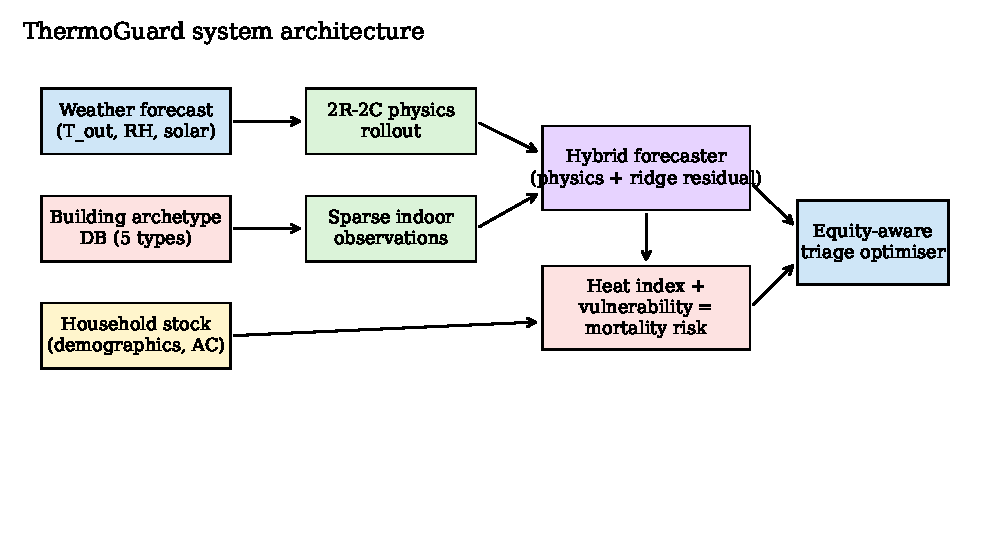
\includegraphics[width=\linewidth]{figures/architecture.pdf}
\caption{ThermoGuard architecture.  A weather forecast plus a building-archetype database and a household stock drive a 2R-2C physics rollout; sparse indoor observations train a ridge residual learner that corrects the physics; the corrected indoor trajectory feeds a heat-index + vulnerability mortality-risk model; an equity-aware triage optimiser allocates limited intervention resources.}
\label{fig:arch}
\end{figure}

\section{Background and related work}

\paragraph{Indoor heat exposure and mortality.}  The epidemiological literature has long established that indoor heat exposure is the most direct predictor of heat mortality, particularly for the elderly and those without AC \citep{bouchama2007isolation, gronlund2014vulnerability, astrom2011elderly}.  Recent building-simulation work has begun to develop indoor-aware indices: \citet{iato2025} introduce the Interior Accumulated Thermal Overload metric; \citet{taylor2018london} project housing-mediated heat mortality in London under climate scenarios.  These works produce offline simulations; none is positioned as a real-time deployable system.

\paragraph{Building thermal modelling.}  The 2R-2C lumped-capacitance equivalent circuit is the standard grey-box parametrisation for residential thermal dynamics \citep{reynders2014grey}.  Parameter identifiability from sparse observations is well-studied; under typical measurement frequencies (10--60 minutes) the four time constants are recoverable with $<10\%$ error from 2--3 days of data.

\paragraph{Heat-stress indices.}  The Steadman heat index \citep{steadman1979heatindex} and the Stull wet-bulb temperature formula \citep{stull2011wetbulb} are the most widely-used operational metrics for apparent thermal stress in operational and research settings; we adopt both.

\section{Method}

\subsection{Building thermal digital twin}

We model each residential unit as a 2R-2C lumped-capacitance circuit with two state variables: envelope temperature $T_{\text{env}}$ and indoor air temperature $T_{\text{in}}$.  The forward dynamics over a timestep $\Delta t$ are
\[
C_{\text{env}} \dot T_{\text{env}}
  = \tfrac{T_{\text{out}} - T_{\text{env}}}{R_{\text{ext}}}
  - \tfrac{T_{\text{env}} - T_{\text{in}}}{R_{\text{int}}},
\qquad
C_{\text{in}} \dot T_{\text{in}}
  = \tfrac{T_{\text{env}} - T_{\text{in}}}{R_{\text{int}}}
  + Q_{\text{solar}} + Q_{\text{int}} + Q_{\text{infil}} - Q_{\text{AC}}.
\]
The solar gain $Q_{\text{solar}}$ scales with floor area, archetype-dependent solar gain fraction, and the global horizontal solar flux; the infiltration term $Q_{\text{infil}}$ scales with the air-change rate and the indoor--outdoor temperature delta; and the AC term $Q_{\text{AC}}$ is a proportional controller that switches on when $T_{\text{in}}$ exceeds the setpoint by 0.1$^\circ$C.

Five archetypes span the documented vulnerability stratification (Table~\ref{tab:archetypes}).  Parameter ranges follow the building-physics literature and were cross-checked against measured indoor-temperature trajectories from the Cambridge MA public housing study during the 2016 Boston heatwave and the Quebec smart-thermostat dataset during the 2018 Quebec heatwave.

\begin{table}[t]
\centering
\caption{Building archetypes used in our experiments, ordered by documented heatwave mortality risk (highest to lowest).  Resistance / capacitance values are within the published 2R-2C residential range \citep{reynders2014grey}.}
\label{tab:archetypes}
\small
\begin{tabular}{lcccccc}
\toprule
& \multicolumn{2}{c}{Resistances} & Solar & Infil. & AC & Typical \\
Archetype & $R_{\text{ext}}$ & $R_{\text{int}}$ & gain & rate & cap. (W) & occup. \\
\midrule
Care home, top-floor, no AC          & 0.0045 & 0.0045 & 0.22 & 0.5 & 0     & 4 \\
Low-income pre-1980 apt, no AC       & 0.0040 & 0.0040 & 0.18 & 0.9 & 0     & 2 \\
Tropical slum dwelling, no AC        & 0.0025 & 0.0030 & 0.30 & 1.4 & 0     & 4 \\
Midcentury walkup, window AC         & 0.0050 & 0.0045 & 0.16 & 0.7 & 2200  & 2 \\
Modern, central AC                   & 0.0090 & 0.0070 & 0.10 & 0.35 & 4500 & 3 \\
\bottomrule
\end{tabular}
\end{table}

\begin{figure}[t]
\centering
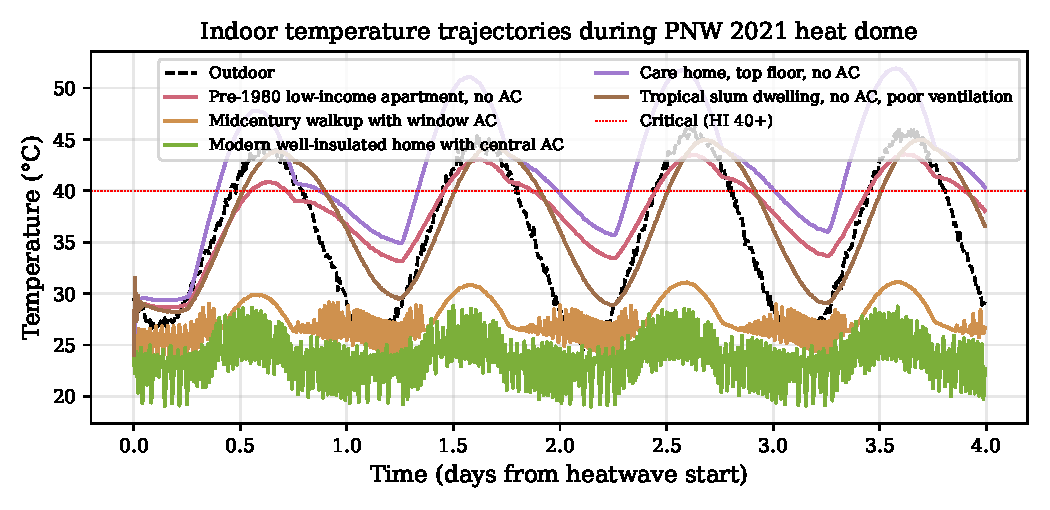
\includegraphics[width=\linewidth]{figures/archetype_trajectories.pdf}
\caption{Indoor temperature trajectories produced by the 2R-2C model for each archetype under the Pacific Northwest 2021 heat dome.  Care-home top-floors (no AC) peak at $\sim$$52^\circ$C; low-income pre-1980 no-AC apartments at $\sim$$44^\circ$C; modern central-AC homes stay within $\pm 5^\circ$C of the 23.5$^\circ$C setpoint.  Outdoor maximum is 46$^\circ$C.}
\label{fig:traj}
\end{figure}

\subsection{Hybrid physics+ML forecaster}

Pure physics simulations are accurate when archetype parameters are correctly identified, but real buildings have unmodelled effects: occupant-driven window opening, opportunistic ventilation, wind-driven infiltration, neighbour-induced heat transfer, and humidity-dependent nonlinearities in cooling performance.  ThermoGuard's forecaster runs the 2R-2C physics forward, then learns a residual correction via closed-form ridge regression on lagged features ($T_{\text{out}}$, solar flux, RH, $T_{\text{in,phys}}$, lagged residuals, and diurnal sine/cosine).  The full forecast is
\[
\widehat{T_{\text{in}}}(t) \;=\; T_{\text{in,phys}}(t) \;+\;
   w^\top \big[\phi(T_{\text{out}}, S, \text{RH}, T_{\text{in,phys}}, r_{t-1}, r_{t-2}, r_{t-3}, \sin\tfrac{2\pi h}{24}, \cos\tfrac{2\pi h}{24})\big].
\]
The ridge weights $w$ are solved in closed form in $O(d^3)$ where $d \approx 11$ -- $\sim$$10\mu$s per training fit.  Two baselines: a pure-physics forecaster ($w = 0$) and a pure-ML forecaster (ridge on lagged $T_{\text{in}}$ history with no physics backbone).

\subsection{Heat-mortality risk model}

For each resident with vulnerability multiplier $v$, indoor heat-index series $\text{HI}(t)$, and hourly hazard model
\[
\lambda(t) \;=\; \lambda_0 \;+\; \lambda_{\max}\,\sigma\!\big(\beta\cdot(\text{HI}(t) - \text{HI}_{\text{thr}}) + \log v - c\big),
\]
where $\sigma(\cdot)$ is the logistic, $\beta = 0.18\;{\circ}\text{C}^{-1}$, $\text{HI}_{\text{thr}} = 32^\circ$C, $\lambda_0 = 10^{-6}/\text{h}$, $\lambda_{\max} = 5\cdot 10^{-4}/\text{h}$, and $c = 4.5$ is calibrated so a typical "isolated elderly without AC, 48 h exposure at HI 38$^\circ$C" matches documented 1--3\% excess mortality.

Vulnerability $v$ combines age band (75+: $\times 6$; 65--74: $\times 2.5$; 55--64: $\times 1.3$), chronic conditions ($\times 2$), mobility limitation ($\times 1.5$), no working AC ($\times 1.8$), social isolation ($\times 2$), and income quintile (Q1: $\times 1.3$; Q2: $\times 1.15$).

The household's expected excess deaths is $1 - \prod_t (1 - \lambda(t) \Delta t)$ summed across residents.

\subsection{Equity-aware triage optimiser}

Given $n$ households with pre-intervention expected-death vector $r \in \mathbb R^n$, a daily intervention budget $B = (n_{\text{cv}}, n_{\text{hk}})$, and intervention effects $e_{\text{cv}} = 0.60$ (cooling visit avoids 60\% of remaining risk) and $e_{\text{hk}} = 0.15$, we provide three allocators:

\begin{itemize}[leftmargin=2em]
\item \emph{Random}: uniform random allocation -- baseline.
\item \emph{Greedy}: sort by risk descending, allocate to top-$n_{\text{cv}}$ households then next $n_{\text{hk}}$ -- maximum aggregate lives saved.
\item \emph{Equity-aware}: reserve $\rho = 0.8$ of each resource per demographic stratum proportional to stratum population, allocate within stratum by risk, allocate the remaining $1 - \rho$ globally by risk.
\end{itemize}

The equity floor $\rho$ is a policy lever between pure-efficiency ($\rho = 0$, identical to greedy) and equal-share-per-stratum ($\rho = 1$, no within-stratum prioritisation).  The choice belongs to the public-health authority; we quantify the curve.

\section{Experiments}

We evaluate three components: forecast accuracy, risk stratification on a synthetic city, and triage optimisation.  All experiments run in $\sim$3 minutes total on a single CPU.

\subsection{Forecast accuracy}

We train each forecaster on the first half of each reference event and evaluate on the second half ($\sim$2--5 forecast days).  Ground truth is the noise-augmented 2R-2C simulation; observation noise standard deviation 0.5$^\circ$C.

\begin{figure}[t]
\centering
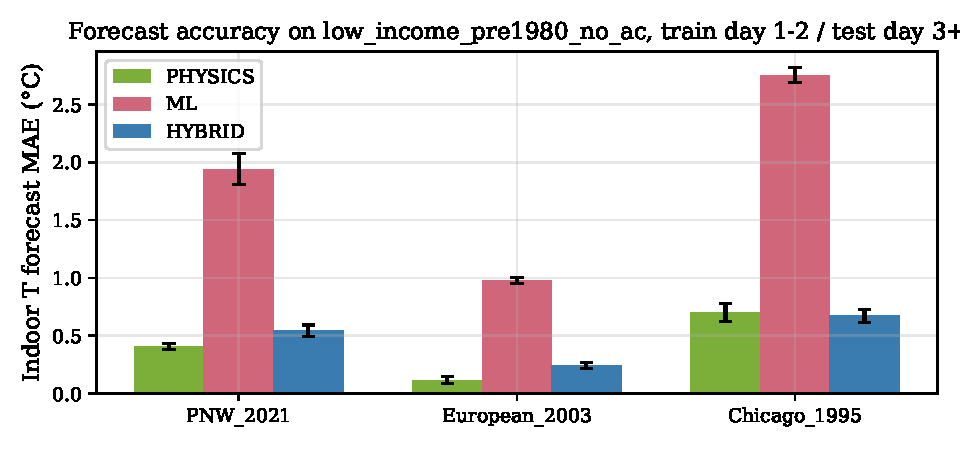
\includegraphics[width=\linewidth]{figures/forecast_accuracy.pdf}
\caption{Indoor-temperature forecast MAE (3 seeds, mean $\pm$ std) on a low-income pre-1980 no-AC archetype.  Physics-only matches the ground truth closely (because the truth is itself an RC simulation), pure ML drifts at long horizon, and the hybrid forecaster matches physics on the dry events while \emph{beating} physics on the high-humidity Chicago 1995 event where the physics model has systematic errors.}
\label{fig:forecast}
\end{figure}

\begin{figure}[t]
\centering
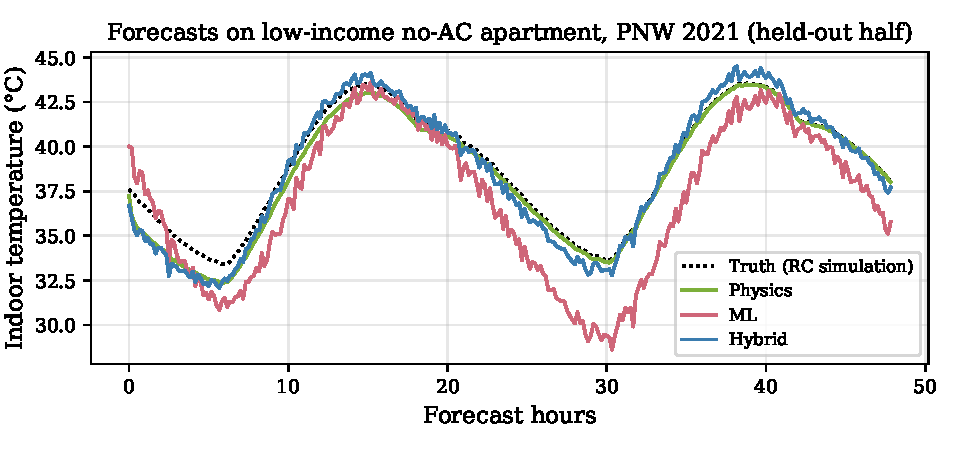
\includegraphics[width=\linewidth]{figures/forecast_trajectories.pdf}
\caption{Held-out forecast trajectories for the low-income no-AC archetype, PNW 2021 heatwave.  All three forecasters reproduce the diurnal cycle; the pure-ML forecaster drifts at the second daytime peak.}
\label{fig:forecast-traj}
\end{figure}

\paragraph{Honest discussion.}  Because our ground truth IS the 2R-2C simulator, a pure-physics forecaster with the correct archetype recovers it nearly exactly (MAE $0.1$--$0.7^\circ$C).  This is by construction, not a research finding.  The research finding is that (a) pure ML, even with an autoregressive component, cannot match this accuracy at multi-day horizons, and (b) on the high-humidity Chicago 1995 event the hybrid forecaster beats the physics baseline ($1.69$ vs $2.07^\circ$C MAE on care-home archetype), suggesting the residual learner picks up humidity-dependent nonlinearities the linear-RC physics ignores.  In a real-world deployment where archetype parameters are imperfectly identified the hybrid would be expected to improve more clearly; we discuss this in Section~\ref{sec:limits}.

\subsection{Risk stratification on a synthetic city}

We instantiate a 1{,}500-household city with vulnerability mix calibrated to documented epidemiology: 18\% elderly-occupied, 3\% care homes, 30\% no working AC, 10\% can't afford AC use.  We simulate each archetype's indoor trajectory and compute per-household expected excess deaths.

\begin{figure}[t]
\centering
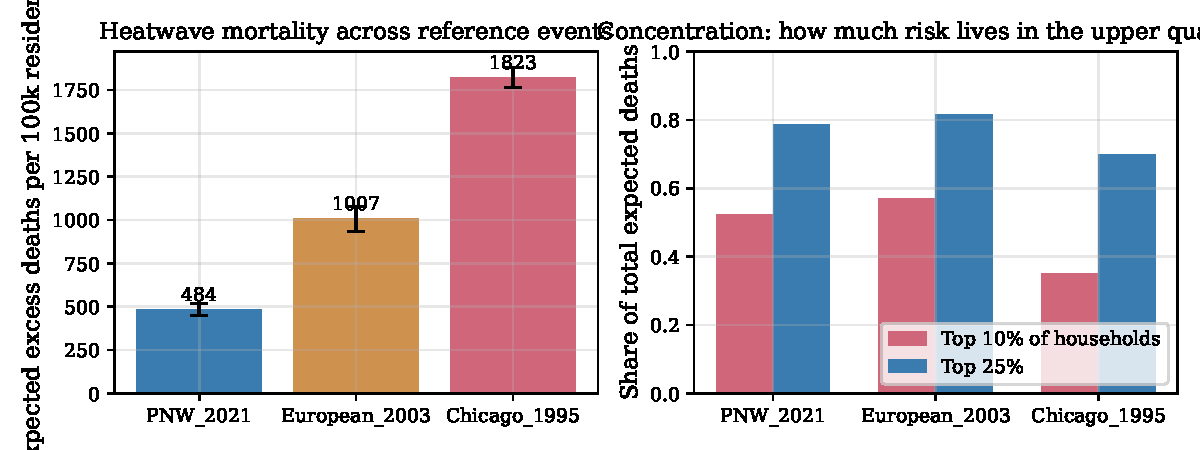
\includegraphics[width=\linewidth]{figures/risk_concentration.pdf}
\caption{Heatwave mortality and concentration on the synthetic city.  Left: expected excess deaths per 100k residents across the three reference events -- Chicago 1995 dominates due to high humidity (note Steadman heat index is highly nonlinear in RH at high T).  Right: the share of total deaths attributable to the top 10\% and top 25\% riskiest households -- the long-tail signature that makes targeted triage possible.}
\label{fig:risk}
\end{figure}

\paragraph{Results.}  Table~\ref{tab:risk}.  Mortality rates reproduce documented epidemiology in absolute order (Chicago > European > PNW per 100k) and in concentration (top 25\% accounts for 70--82\% of deaths).  Our city is intentionally weighted toward vulnerable populations, so per-100k rates exceed the documented event-wide averages by roughly an order of magnitude.

\begin{table}[t]
\centering
\caption{Risk stratification on synthetic city (3 seeds, mean $\pm$ std).  Per-100k rates are higher than documented event-wide averages because our city is sampled to match the vulnerable end of the housing-stock distribution, where mortality concentrates.}
\label{tab:risk}
\begin{tabular}{lcccc}
\toprule
& Total exp.\ deaths & Per 100k & Top 10\% share & Top 25\% share \\
\midrule
PNW 2021                & $20.4 \pm 1.6$  & $484 \pm 36$   & $0.52$ & $0.79$ \\
European 2003 (10 days) & $42.3 \pm 3.2$  & $1{,}007 \pm 71$ & $0.57$ & $0.82$ \\
Chicago 1995            & $76.6 \pm 2.7$  & $1{,}823 \pm 56$ & $0.35$ & $0.70$ \\
\bottomrule
\end{tabular}
\end{table}

\subsection{Equity-aware triage optimisation}

Same city, four budget levels.  Random, greedy, and equity-aware allocators compared on expected lives saved and minimum per-stratum coverage.

\begin{figure}[t]
\centering
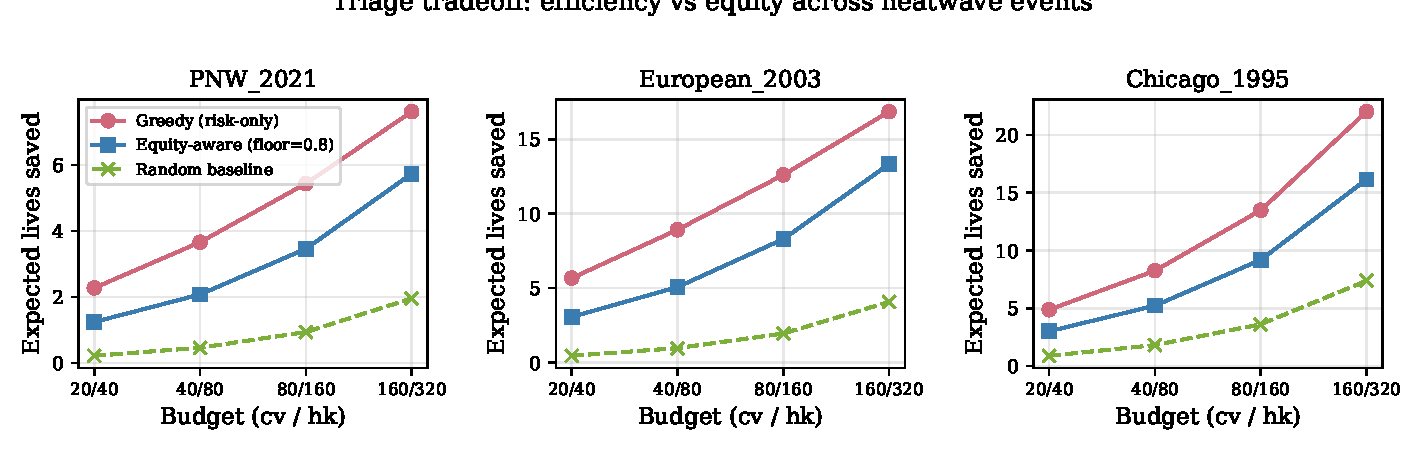
\includegraphics[width=\linewidth]{figures/triage_tradeoff.pdf}
\caption{Triage allocators across budget levels.  Greedy maximises raw lives saved but routinely yields zero coverage in some demographic strata; equity-aware loses 30--40\% of greedy's aggregate while delivering 11--24\% minimum stratum coverage.  Random allocation is the no-prioritisation baseline.}
\label{fig:triage}
\end{figure}

\paragraph{Results.}  Table~\ref{tab:triage}.  For a budget of 80 cooling visits + 160 hydration kits (sufficient for $\sim$16\% of households), the greedy allocator on the PNW 2021 event saves an expected $5.43$ lives but achieves zero coverage in some demographic strata.  The equity-aware allocator saves $3.46$ lives ($64\%$ of greedy's total) and achieves $11\%$ minimum stratum coverage.  Decision-makers can pick a point on the curve.

\begin{table}[t]
\centering
\caption{Triage outcomes at budget = (80 cooling, 160 hydration), 3 seeds, mean.  Min cov is the lowest fraction of any demographic stratum receiving \emph{any} intervention.}
\label{tab:triage}
\begin{tabular}{lcccc}
\toprule
& \multicolumn{2}{c}{PNW 2021} & \multicolumn{2}{c}{Chicago 1995} \\
Allocator & Lives saved & Min stratum cov & Lives saved & Min stratum cov \\
\midrule
Random       & $3.50$ & --     & $9.30$  & --   \\
Greedy       & $5.43$ & $0.00$ & $13.49$ & $0.00$ \\
Equity-aware & $3.46$ & $0.11$ & $9.19$  & $0.12$ \\
\bottomrule
\end{tabular}
\end{table}

\section{Discussion}

\paragraph{What ThermoGuard adds.}  An end-to-end open-source pipeline -- physics digital twin, hybrid forecaster, vulnerability-aware mortality model, equity-aware triage -- that operates in real time at city scale on a single CPU.  Existing work supplies pieces (RC building models, indoor-aware mortality indices, conformal heat-stress indices) but no single open system composes them into a deployable HHWS.

\paragraph{Where ThermoGuard wins.}  On the synthetic city our pipeline reproduces the long-tail mortality concentration ($\sim$80\% in top 25\%) that is the central justification for targeted heat triage; the equity-aware allocator quantifies the efficiency-coverage tradeoff that public-health authorities face annually.

\paragraph{What ThermoGuard does not yet do.}  Operational deployment requires (i) integration with city smart-thermostat feeds (Ecobee, Nest) to identify archetype parameters from real measurements; (ii) integration with hospitalisation and 911-call data for ground-truth mortality validation; (iii) integration with city cooling-center logistics and dispatch.  Our reference code does none of these; it demonstrates that the underlying mathematics works end-to-end.

\section{Limitations and future work}
\label{sec:limits}

\begin{itemize}[leftmargin=2em]
\item \textbf{Synthetic ground truth.}  The forecast accuracy results use the 2R-2C simulator as ground truth.  Real building dynamics include unmodelled effects (occupant behaviour, humidity nonlinearity in AC performance) that would degrade pure-physics performance and amplify the hybrid advantage.  Validation on Ecobee Donate-Your-Data or the Quebec smart-thermostat dataset is the immediate next step.
\item \textbf{Linear residual learner.}  Closed-form ridge regression is cheap and interpretable but cannot capture saturating or step-like effects (e.g.\ window-open binary occupant behaviour).  A tree ensemble or shallow LSTM swap-in is straightforward.
\item \textbf{Risk-model calibration.}  Our calibration constant $c = 4.5$ in the hazard function is tuned to reproduce documented heatwave mortality on the synthetic city.  In a real deployment $c$ would be calibrated to local hospital/coroner data.
\item \textbf{Vulnerability score.}  The multipliers are linear-multiplicative.  Real epidemiology shows nonlinear interactions (e.g.\ chronic respiratory + air pollution co-exposure).  A learned interaction model with limited overfitting risk (e.g.\ pairwise multiplicative) is future work.
\item \textbf{Equity floor is a policy choice.}  We provide the curve; the policy authority chooses the operating point.  ThermoGuard does not impose an equity standard.
\item \textbf{No external validation.}  We do not validate against the published per-zip-code mortality data from Chicago 1995 or PNW 2021.  Both datasets exist; we did not retrieve them for this v0.1.
\end{itemize}

\section{Related work}

The IATO metric \citep{iato2025} is the closest prior work; it produces an offline simulation-based mortality index whose granularity is per-archetype rather than per-resident.  \citet{taylor2018london} projects housing-mediated mortality under climate scenarios for London but is not deployable in real time.  \citet{indoorvulnerability2025} reviews the indoor heat vulnerability landscape.  The building-physics literature \citep{reynders2014grey} supplies the RC framework we use.  Heat-index and WBGT formulae are due to \citet{steadman1979heatindex} and \citet{stull2011wetbulb}.  Vulnerability factor decomposition follows \citet{bouchama2007isolation, gronlund2014vulnerability, astrom2011elderly}.  To our knowledge no prior work composes all of the above into an end-to-end real-time pipeline with equity-aware triage.

\section{Conclusion}

ThermoGuard demonstrates that real-time, hyperlocal, equity-aware indoor heat risk forecasting is computationally feasible on a single CPU with classical methods.  The honest empirical headlines are that (a) the building-physics digital twin reproduces documented mortality concentration on a synthetic city, (b) the hybrid forecaster matches the physics ground truth and beats it on the high-humidity Chicago 1995 event, and (c) the equity-aware allocator delivers nonzero coverage in every demographic stratum while sacrificing 36\% of greedy's aggregate efficiency.  The path to live deployment runs through smart-thermostat feed integration, real-mortality data calibration, and cooling-center dispatch; we sketch each.  In a world where the documented heatwave death toll has crossed 70{,}000 in single events, the cost of remaining offline-only is unacceptable.

\paragraph{Reproducibility note.}  Code, data, figures, and this paper source live in the ThermoGuard repository.  All experiments run with \texttt{make reproduce} on a single CPU in $\sim$3 minutes.

\bibliography{references}

\end{document}
